% mainfile: ../../main.tex
\chapter{Reconstruction by frequency-comb time-domain simulation}\label{ch:ff:validation}
For a given interaction-picture quantum operation $\ev*{\liouvUe}$ resulting from the quantum system's evolution under the noise fully characterized by its one-sided \gls{psd} $S(\omega)$, we \emph{define} the \gls{ff} \FFot by
\begin{align}\label{eq:ff:filter_function:definition}
    \ev*{\liouvUe(\tau)} = \exp\cumulantfun(\tau) = \exp\left\{-\int\frac{\dd{\omega}}{2\pi}\FFot S(\omega)\right\}.
\end{align}
Now, suppose that
\begin{equation}\label{eq:ff:psd:monochromatic}
    S(\omega) = 2\pi\sigma_i^2 \delta(\omega - \omega_i) \eqqcolon S_i(\omega),
\end{equation}
that is, the \gls{psd} of a monochromatic sinusoid of frequency $\omega_i$ and \gls{rms} $\sigma_i$\marginnote{
    \Cref{eq:ff:psd:monochromatic} discretizes $S(\omega)$ by sampling it at points $\omega_i$, \ie,
    \begin{align*}
        S(\omega) \sim \lim_{n\to\infty}\sum_{i=1}^n S_i(\omega).
    \end{align*}
}.
Then \cref{eq:ff:filter_function:definition} becomes
\begin{equation}\label{eq:ff:filter_function:monochromatic}
    \begin{split}
        \ev*{\liouvUe_i(\tau)} =& \exp\left\lbrace -2\pi\sigma_i^2\int\frac{\dd{\omega}}{2\pi}\FFot\delta(\omega - \omega_i)\right\rbrace \\
                               =& \exp\left\lbrace -\sigma_i^2\mc{F}(\omega_i;\tau)\right\rbrace,
    \end{split}
\end{equation}
where $\ev*{\liouvUe_i(\tau)}$ is the noisy quantum operation generated by monochromatic noise with \gls{psd} $S_i(\omega)$ according to \cref{eq:ff:psd:monochromatic}.
It is now easy to invert \cref{eq:ff:filter_function:monochromatic}, and we obtain
\begin{align}\label{eq:ff:filter_function:monochromatic:solved}
    \mc{F}(\omega_i; \tau) = -\sigma_i^{-2}\log\ev*{\liouvUe_i(\tau)}.
\end{align}
Because we represent quantum operations as matrices in Liouville space, \cref{eq:ff:filter_function:monochromatic:solved} is easy to implement on a computer; to sample the exact \gls{ff} at the set of discrete frequencies $\lbrace\omega_i\rbrace_i$ we simply need to compute $\liouvUe_i(\tau)$  using a time-domain simulation method of our choice and take the logarithm!\sidenote{A similar approach was pursued by \citeauthor{Geck2021} in her PhD thesis to compare gate fidelities~\cite{Geck2021}.}

Indeed, we can go a step further and split apart the coherent and incoherent contributions to the noisy evolution.
Since (in-)coherent quantum operations are represented by (anti-)symmetric matrices in Liouville space, we may define the incoherent and coherent \glspl{ff} by
\begin{equation}\label{eq:ff:filter_function:monte_carlo:incoherent}
    \begin{split}
        \mc{F}_\decayamps(\omega_i;\tau) =& \frac{1}{2}\left(\mc{F}(\omega_i;\tau) + \mc{F}(\omega_i;\tau)\transpose\right) \\
                                         =& \frac{1}{2\sigma_i^2}\left(\log\ev*{\liouvUe_i(\tau)} + \log\ev*{\liouvUe_i(\tau)}\transpose\right),
    \end{split}
\end{equation}
and
\begin{equation}\label{eq:ff:filter_function:monte_carlo:coherent}
    \begin{split}
        \mc{F}_\freqshifts(\omega_i;\tau) =& \frac{1}{2}\left(\mc{F}(\omega_i;\tau) - \mc{F}(\omega_i;\tau)\transpose\right) \\
                                          =& \frac{1}{2\sigma_i^2}\left(\log\ev*{\liouvUe_i(\tau)} - \log\ev*{\liouvUe_i(\tau)}\transpose\right),
    \end{split}
\end{equation}
respectively.
This allows us to analyze in detail deviations of the closed-form expression obtained by means of the cumulant expansion \todo{ref}, from the exact filter functions given by \cref{eq:ff:filter_function:monte_carlo:coherent,eq:ff:filter_function:monte_carlo:incoherent}.
In the following, I will lay out explicitly how these can be computed in the time domain.

To begin with, observe that from a \gls{mc} point of view, \liouvUe is given by
\begin{align}
    \liouvUe(\tau) \equiv \expval{\liouvUe_i(\tau)} = \liouvQ\transpose \expval{\liouvU_i(\tau)},
\end{align}
where $\liouvU_i(\tau)$ is the solution of the Schrödinger equation for a single realization of the noise and $\expval{\placeholder}$ denotes the ensemble average\marginnote{
    For $N$ realizations of the stochastic process underlying $b(t)$, the ensemble average of a quantity $A(t)$ that is a function of $b(t)$ is given by
    \begin{align*}
        \expval{A}(t) = \frac{1}{N}\sum_{i=1}^N A_i(t)
    \end{align*}
    where $i$ enumerates the realizations of the stochastic process.
    The relative error of this average scales as $N^{-\flatfrac{1}{2}}$.
}.
Inserting into \cref{eq:ff:filter_function:monochromatic}, we find
\begin{equation}
    \label{eq:ff:filter_function:monte_carlo}
    \begin{split}
        \mc{F}(\omega_i; \tau) =& \sigma_i^{-2}\log\expval{\liouvUe_i(\tau)} \\
                               =& \sigma_i^{-2}\log\liouvQ\transpose\expval{\liouvU_i(\tau)}.
    \end{split}
\end{equation}
If we evaluate \cref{eq:ff:filter_function:monte_carlo} for a set of frequencies $\lbrace\omega_i\rbrace_i$ sampling the true spectrum $S(\omega)$ sufficiently well, we thus obtain the exact filter function \FF (within the accuracy of \gls{mc}), allowing us to compare the accuracy of the formalism developed in\todo{ref}.

So what does a single noise realization of \cref{eq:ff:psd:monochromatic} in the time domain look like? \todo{tikz sketch?}
It's a sinusoid with amplitude $A_i \sim\rayleigh(\sigma_i)$,\sidenote{
    $\rayleigh(\sigma)$ is the Rayleigh distribution with probability density function \cite{RayleighDistributionWiki}
    \begin{equation*}
        \rho(x) = \frac{x}{\sigma^2}\exp{-\frac{x^2}{2\sigma^2}}.
    \end{equation*}
    It describes the probability distribution of the distance from the origin of a point drawn from a bivariate normal distribution with mean $0$ and standard deviation $\sigma$.
}
frequency $\omega_i$, and phase $\phi \sim \uniform(0, 2\pi)$,\sidenote{
    The probability density function of the uniform distribution $\uniform(a, b)$ is
    \begin{equation*}
        \rho(y) = \begin{cases}
        (b - a)^{-1}    & \qif* a\leq y < b, \\
        0               & \qelse*
        \end{cases}
    \end{equation*}
}
\begin{equation}\label{eq:ff:monte_carlo:noise_trace}
    b(t) = A_i\sin(\omega_i t + \phi).
\end{equation}
Instead of taking the random sampling approach of \gls{mc}, we can also compute the expectation value of $\liouvU_i(t)$ over $A_i$ and $\phi$ by integrating over the probability density functions,\sidenote{
    We write the expectation value of an observable $A$ with respect to a random variable $X$ with the probability density function $\rho_X$ as $\mathbb{E}_X[A]$.
}
\begin{equation}
    \label{eq:ff:monte_carlo:propagator:average}
    \mathbb{E}_{A_i,\phi}[\liouvU] = \int\dd{x}\rho_{A_i}(x)\int\dd{y}\rho_{\phi}(y)\liouvU[x, y],
\end{equation}
where we wrote $\liouvU[x, y]$ for the Liouville representation of the \gls{mc} propagator for single $x$ and $y$ drawn from their respective distributions.
Whether we choose the \gls{mc} method or direct integration, in practice \cref{eq:ff:monte_carlo:propagator:average} will be evaluated numerically, either by drawing random samples from the distributions $\text{Rice}(0, \sigma_i)$ and $U(0,2\pi)$ or by discretizing \cref{eq:ff:monte_carlo:propagator:average}.

\begin{figure}
    \centering
    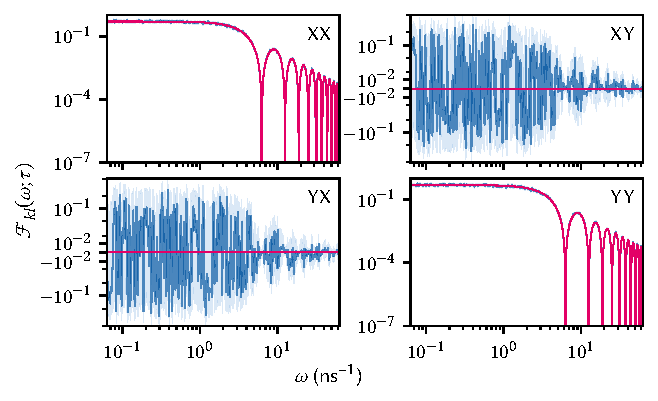
\includegraphics{img/pdf/filter_functions/monte_carlo_FF_Z}
    \caption[\imgsource{img/py/filter_functions/monte_carlo_filter_functions.py}]{}
    \label{fig:ff:monte_carlo:Z}
\end{figure}

\begin{figure*}
    \centering
    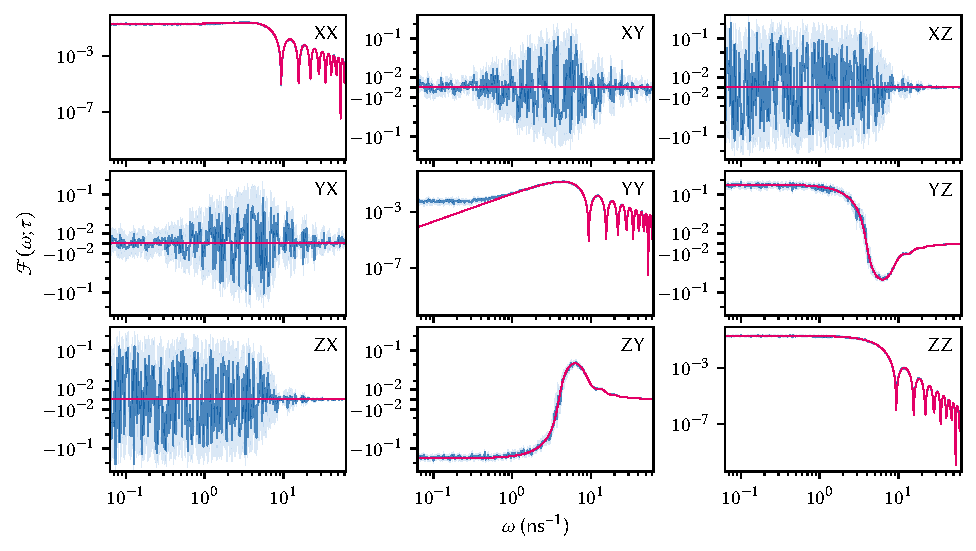
\includegraphics{img/pdf/filter_functions/monte_carlo_FF_X}
    \caption[\imgsource{img/py/filter_functions/monte_carlo_filter_functions.py}]{}
    \label{fig:ff:monte_carlo:X}
\end{figure*}

\begin{figure*}
    \centering
    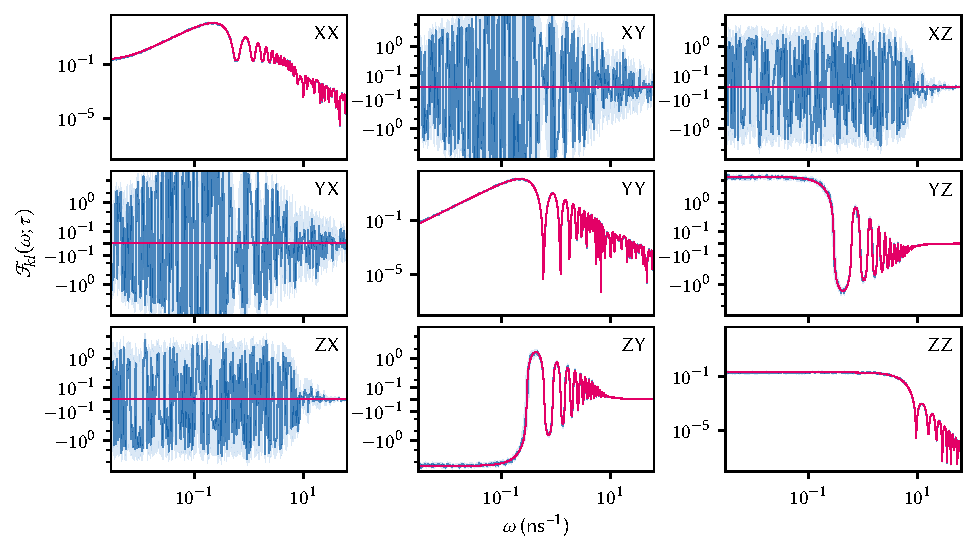
\includegraphics{img/pdf/filter_functions/monte_carlo_FF_spin_echo}
    \caption[\imgsource{img/py/filter_functions/monte_carlo_filter_functions.py}]{}
    \label{fig:ff:monte_carlo:echo}
\end{figure*}
